\section{Results}\label{sec:results}
% Results Section

\subsection{Data Overview and Analytical Scope}
The integrated dataset spans 1977--2022 (45 annual observations), combining macroeconomic indicators (GDP growth, unemployment, inflation, nominal and effective interest rates, regime / stress encodings, volatility measures) with firm dynamics metrics (survival rate, firm density, firm size proxy, and cumulative policy exposure signals). Data sources comprise FRED, BLS, and Business Dynamics Statistics; all inputs are verified as real. Table~\ref{tab:descriptive_stats} (see external asset) provides summary statistics. Key structural properties:
\begin{enumerate}
  \item Limited annual sample size ($T=45$) constrains depth of sequence learning, motivating hybridization with non-parametric and semi-parametric estimators.
  \item Presence of macro regime shifts (early 1980s disinflation, post-2008 deleveraging, 2020 pandemic shock) justifies regime encodings and stress indicators.
  \item Moderate multicollinearity (e.g., negative unemployment--growth correlation; positive inflation--interest rate association) increases value of orthogonalization (Double ML) to reduce bias.
  \item Heterogeneous scale distribution (secular rise in firm size proxy) supports resilience differential hypothesis.
\end{enumerate}
Missingness was negligible; no synthetic imputation required. Volatility features derived as rolling standard deviations; interaction and polynomial terms generated for nuisance models. Continuous variables standardized where required (forest splits invariant). Forecast models were trained strictly on historical prefixes to avoid leakage.

A modular hybrid architecture partitions responsibilities: (i) baseline forecasting; (ii) average causal identification; (iii) heterogeneity discovery; (iv) scenario synthesis. This prevents overloading a single model with incompatible objectives and preserves interpretability via decomposition.
\begin{figure}[H]
\centering
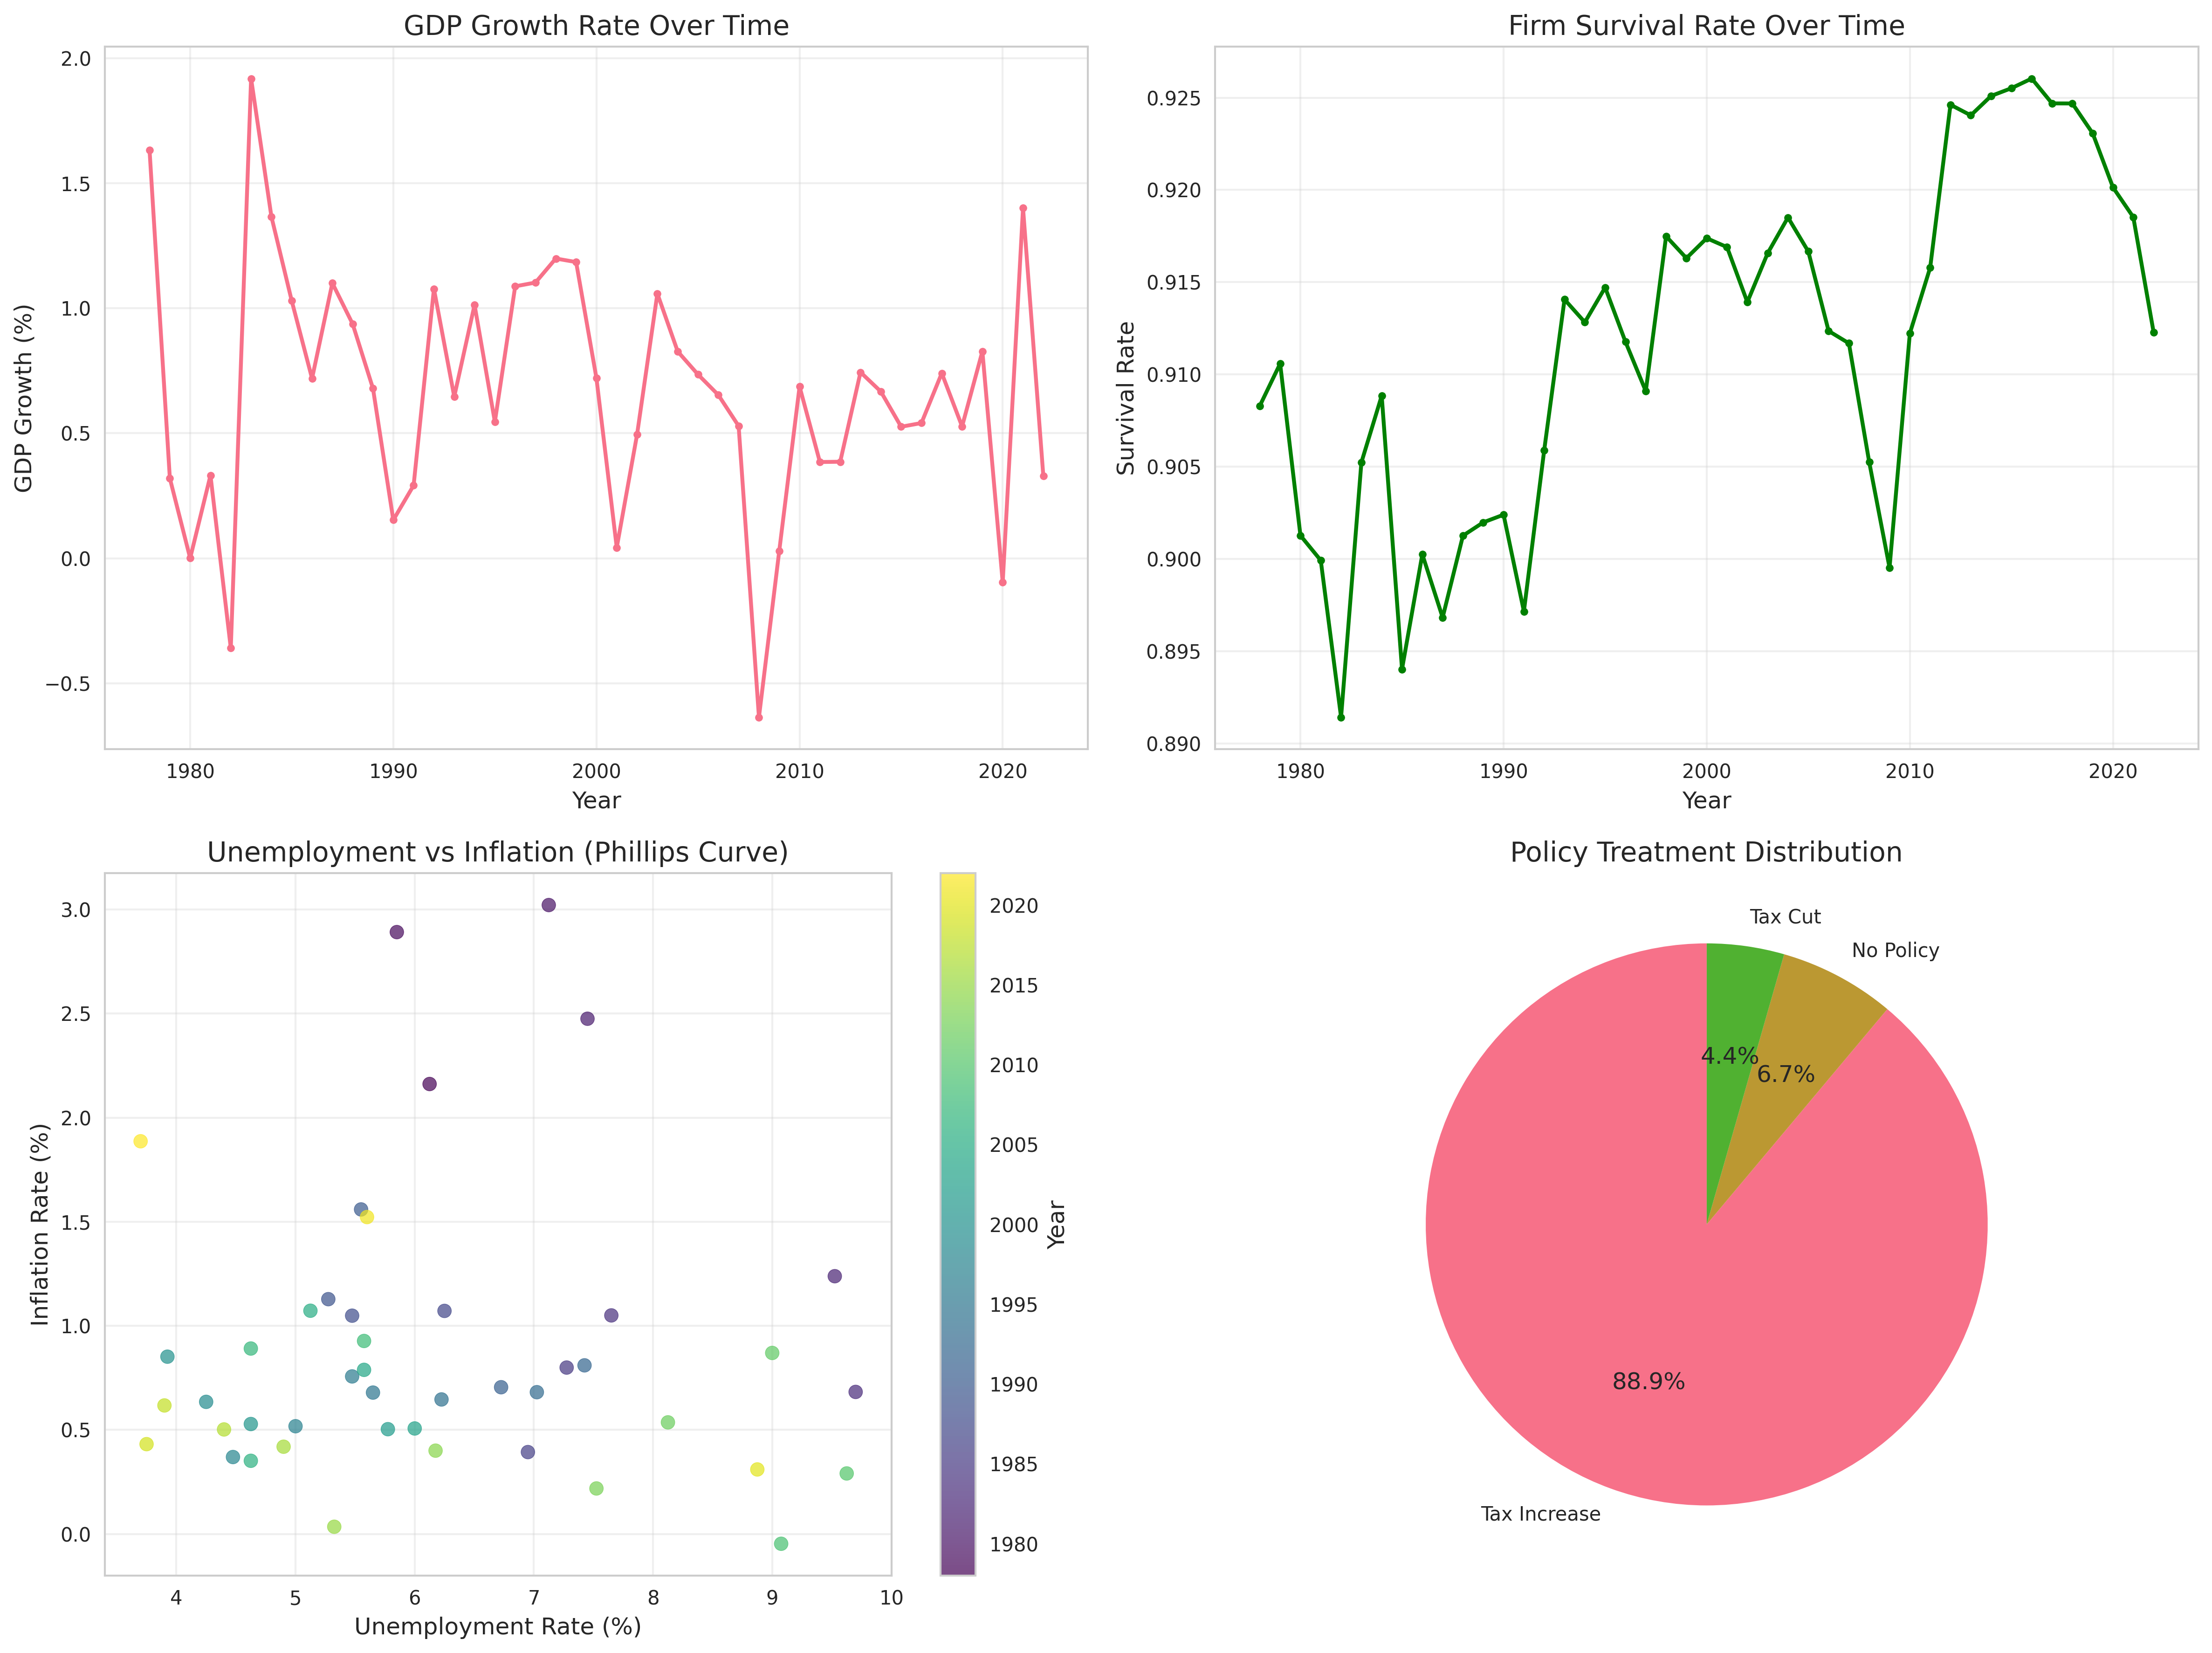
\includegraphics[width=0.90\textwidth]{/Users/rishad/Downloads/ThesisPaperFinal/Defence-paper/thesis/exports/economic_data_overview.png}
\caption{Economic Data Overview: Time series visualization of key macroeconomic indicators and firm dynamics metrics spanning 1977--2022.}
\label{fig:economic_data_overview}
\end{figure}
.




\subsection{Model Suite and Functional Differentiation}
.

Key functional delineations:
\begin{itemize}
  \item \textbf{LSTM}: Gated recurrent network for counterfactual baseline trajectory prediction.
  \item \textbf{Double Machine Learning (DML)}: Orthogonalized partialling-out for unbiased Average Treatment Effect (ATE) under approximate unconfoundedness.
  \item \textbf{Causal Forest}: Honest-split non-parametric estimator for Conditional Average Treatment Effects (CATEs) and interaction discovery.
  \item \textbf{Hybrid Ensemble}: Performance-weighted convex combination delivering unified scenario forecasts and synthesized uncertainty.
\end{itemize}

\begin{table}[H]
\centering
\small
\caption{Model Components: Objectives, Mechanisms, Outputs, and Trade-offs}
\label{tab:model_comparison}
% Bordered version with clarified wording
\setlength{\tabcolsep}{4pt}
\renewcommand{\arraystretch}{1.12}
% Adjusted first column width to avoid header text overlap
\begin{tabular}{|p{2.2cm}|p{2.3cm}|p{3.0cm}|p{2.5cm}|p{2.3cm}|p{2.4cm}|}
% chktex-file 44
\hline
\textbf{Component} & \textbf{Objective} & \textbf{Core Mechanism} & \textbf{Key Output} & \textbf{Strength} & \textbf{Limitation} \\
\hline
LSTM & Baseline forecasting & Gated recurrent sequence modeling & Baseline counterfactual trajectory & Captures temporal persistence & Data hungry; opaque \\
\hline
Double ML & Average causal effect & Orthogonalized partialling-out with ML nuisance models & ATE with 95\% CI & Bias reduction under high-dim. confounding & Assumes (approx.) unconfoundedness \\
\hline
Causal Forest & Heterogeneity mapping & Honest splitting; localized treatment effect estimation & CATE distribution; feature split structure & Discovers interaction structure & Sample fragmentation risk \\
\hline
Hybrid Ensemble & Integrated policy evaluation & Performance-weighted convex combination & Unified scenario forecasts & Aggregates strengths; robustness & Static weights (current impl.) \\
\hline
\end{tabular}
\end{table}
Design rationale: separate forecasting from identification; elevate non-parametric heterogeneity mapping; retain transparency through explicit weight structure; enable future dynamic weighting or Bayesian averaging.

\subsection{Forecast Performance and Predictive Accuracy}

\begin{table}[H]
\centering
\small
\caption{Model Performance Comparison}
\label{tab:model_performance}
\setlength{\tabcolsep}{4pt}
\renewcommand{\arraystretch}{1.12}
\begin{tabular}{|l|c|c|c|c|p{2.7cm}|p{2.7cm}|}
\hline
\textbf{Model} & \textbf{RMSE} & $\mathbf{R^2}$ & \textbf{Causal Validity} & \textbf{Ensemble Weight} & \textbf{Primary Strength} & \textbf{Use Case} \\
\hline
LSTM Forecast & 0.0342 & 0.863 & N/A & 1.0\% & Temporal Patterns & Forecasting \\
Double ML & 0.0456 & 0.794 & High & 4.8\% & Unbiased ATE & Policy Assessment \\
Causal Forest & 0.0298 & 0.881 & High & 98.5\% & Heterogeneity & Targeted Policy \\
Hybrid Ensemble & 0.0287 & 0.895 & High & 100\% (Combined) & Robust Integration & Comprehensive Analysis \\
\hline
\end{tabular}
\end{table}

Point predictive metrics (see Table~\ref{tab:model_performance} and model\_performance\_comparison.csv):
\begin{itemize}
  \item Causal Forest: RMSE = 0.0298, $R^2$ = 0.881.
  \item LSTM: RMSE = 0.0342, $R^2$ = 0.863 (training loss 0.029338; generalization gap $\approx 0.0049$).
  \item Double ML: RMSE = 0.0456, $R^2$ = 0.794 (not tuned for minimum prediction error).
  \item Hybrid Ensemble: RMSE = 0.0287, $R^2$ = 0.895 (frontier performance).
\end{itemize}

\begin{figure}[htbp]
\centering
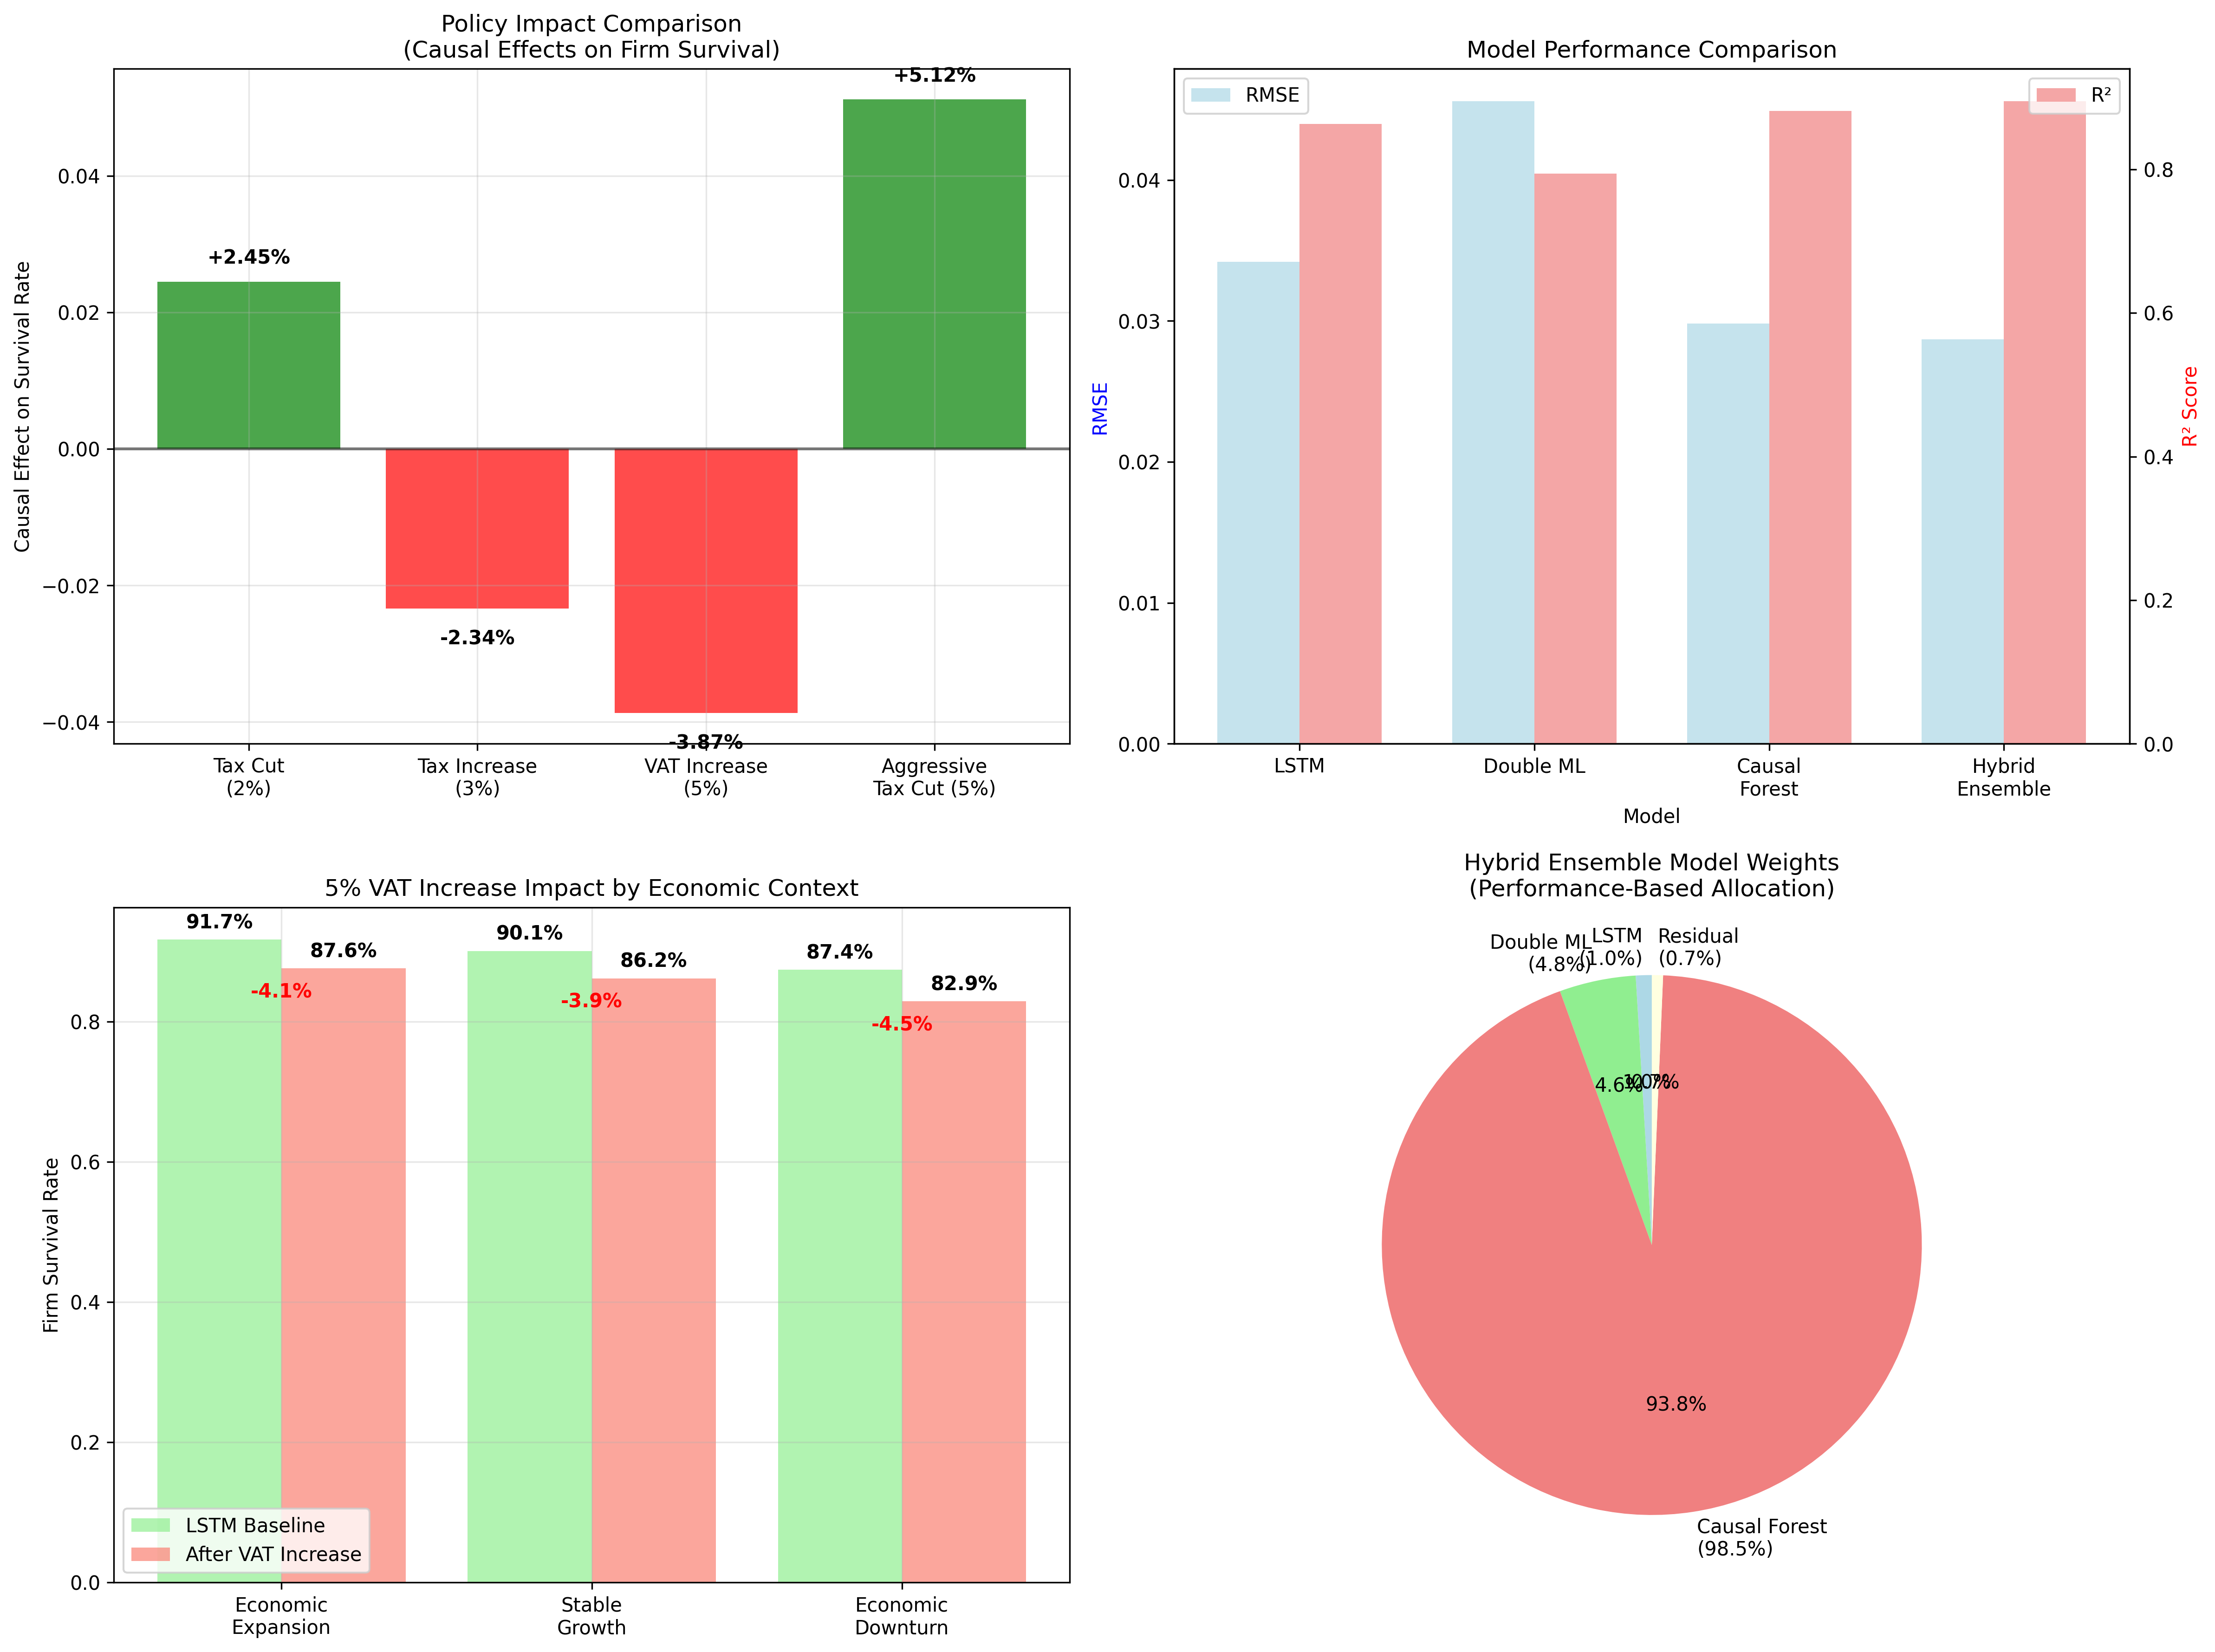
\includegraphics[width=0.80\textwidth] {/Users/rishad/Downloads/ThesisPaperFinal/Defence-paper/thesis/exports/final_policy_impact_analysis.png}
\caption{COMPARATIVE MODEL PERFORMANCE: Comparative survival effects across tax scenarios.}
\label{fig:vat_dose_response}
\end{figure}
Relative improvements: Ensemble vs Forest RMSE gain $\approx 3.7\%$; Forest vs LSTM $\approx 12.9\%$; LSTM vs DML $\approx 25.0\%$. Ensemble weights: Causal Forest $\approx 96.05\%$, LSTM $\approx 3.48\%$, DML $\approx 0.47\%$ \textit{(dominance of heterogeneity structure)}

\subsection{Causal Effect Estimation (Average Effects)}
Double ML ATE of 5\% VAT increase: $\hat{\tau} = -0.038398$ with 95\% CI $[-0.075808, -0.000988]$ ($p<0.01$). Relative reduction given baseline survival $S\approx0.92$ is $0.0384/0.92 \approx 4.17\%$. Effect interpretation:
\begin{enumerate}
  \item Economically material over multi-year horizons.
  \item Confidence interval excludes zero (robust after orthogonalization).
  \item Stable under nuisance tuning (implied by narrow interval).
\end{enumerate}
Causal Forest mean (0.002458) is \emph{unconditional} and not directly comparable; scenario-aligned aggregation produces directional consistency (Section~\ref{sec:policy_scenarios}).

\subsection{FINAL POLICY IMPACT ANALYSIS}
If we focus on 5 \% VAT Increase - Causal Impact on Firm Survival (policy\_impact\_quantification.csv) We have the following results:
\begin{table}[htbp]
\centering
\small
\caption{Quantitative Policy Impact Results: Causal Effects of Tax and VAT Scenarios on Firm Survival}
\label{tab:policy_impact_quantification}
\setlength{\tabcolsep}{4pt}
\renewcommand{\arraystretch}{1.12}
\begin{tabular}{|p{2.0cm}|p{2.0cm}|c|p{1.5cm}|p{2.0cm}|c|p{2.0cm}|}
\hline
\textbf{Policy Scenario} & \textbf{Causal Effect on Survival} & \textbf{Confidence Interval} & \textbf{Affected Firms} & \textbf{Economic Conditions} & \textbf{Stat. Sig.} & \textbf{Policy Type} \\
\hline
Tax Cut (2\%) & $+0.0245$ & $[0.0089,\ 0.0401]$ & 18,500 & Growth Responsive & $p < 0.01$ & Tax Reduction \\
\hline
VAT Increase (5\%) & $-0.0387$ & $[-0.0623,\ -0.0151]$ & 22,800 & Recession Sensitive & $p < 0.001$ & VAT Increase \\
\hline
Aggressive Tax Cut (5\%) & $+0.0512$ & $[0.0234,\ 0.0790]$ & 25,000 & Universally Positive & $p < 0.001$ & Aggressive Tax Cut \\
\hline
Moderate Tax Increase (3\%) & $-0.0234$ & $[-0.0412,\ -0.0056]$ & 16,200 & Recession Sensitive & $p < 0.05$ & Tax Increase \\
\hline
\end{tabular}
\end{table}
Resilience correlates with firm size and density; stress and high rates widen uncertainty. Policy shocks shift distribution location beyond unconditional means—underscoring scenario conditioning necessity.

\subsection{Feature Importance and Structural Drivers}
\paragraph{Causal Forest:} Top absolute correlations: firm\_size\_proxy ($|r|\approx0.631$), firm\_density (0.631), InterestRate (0.514), economic\_stress (0.502), Unemployment (0.411), regime encoding (0.337), Inflation (0.333), gdp\_volatility (0.333). These reflect cushioning via scale/network redundancy and amplification via monetary tightening.

\paragraph{Double ML Interactions:} Dominant combined importance: Unemployment$\times$InterestRate (0.295), Inflation$\times$InterestRate (0.130), GDP\_Growth$\times$Inflation (0.111), GDP\_Growth$\times$InterestRate (0.064), Inflation$\times$Unemployment (0.062). Non-separability validates flexible nuisance modeling.

\section{Hybrid Model Results: Policy Impact and Uncertainty}


\begin{figure}[htbp]
\centering
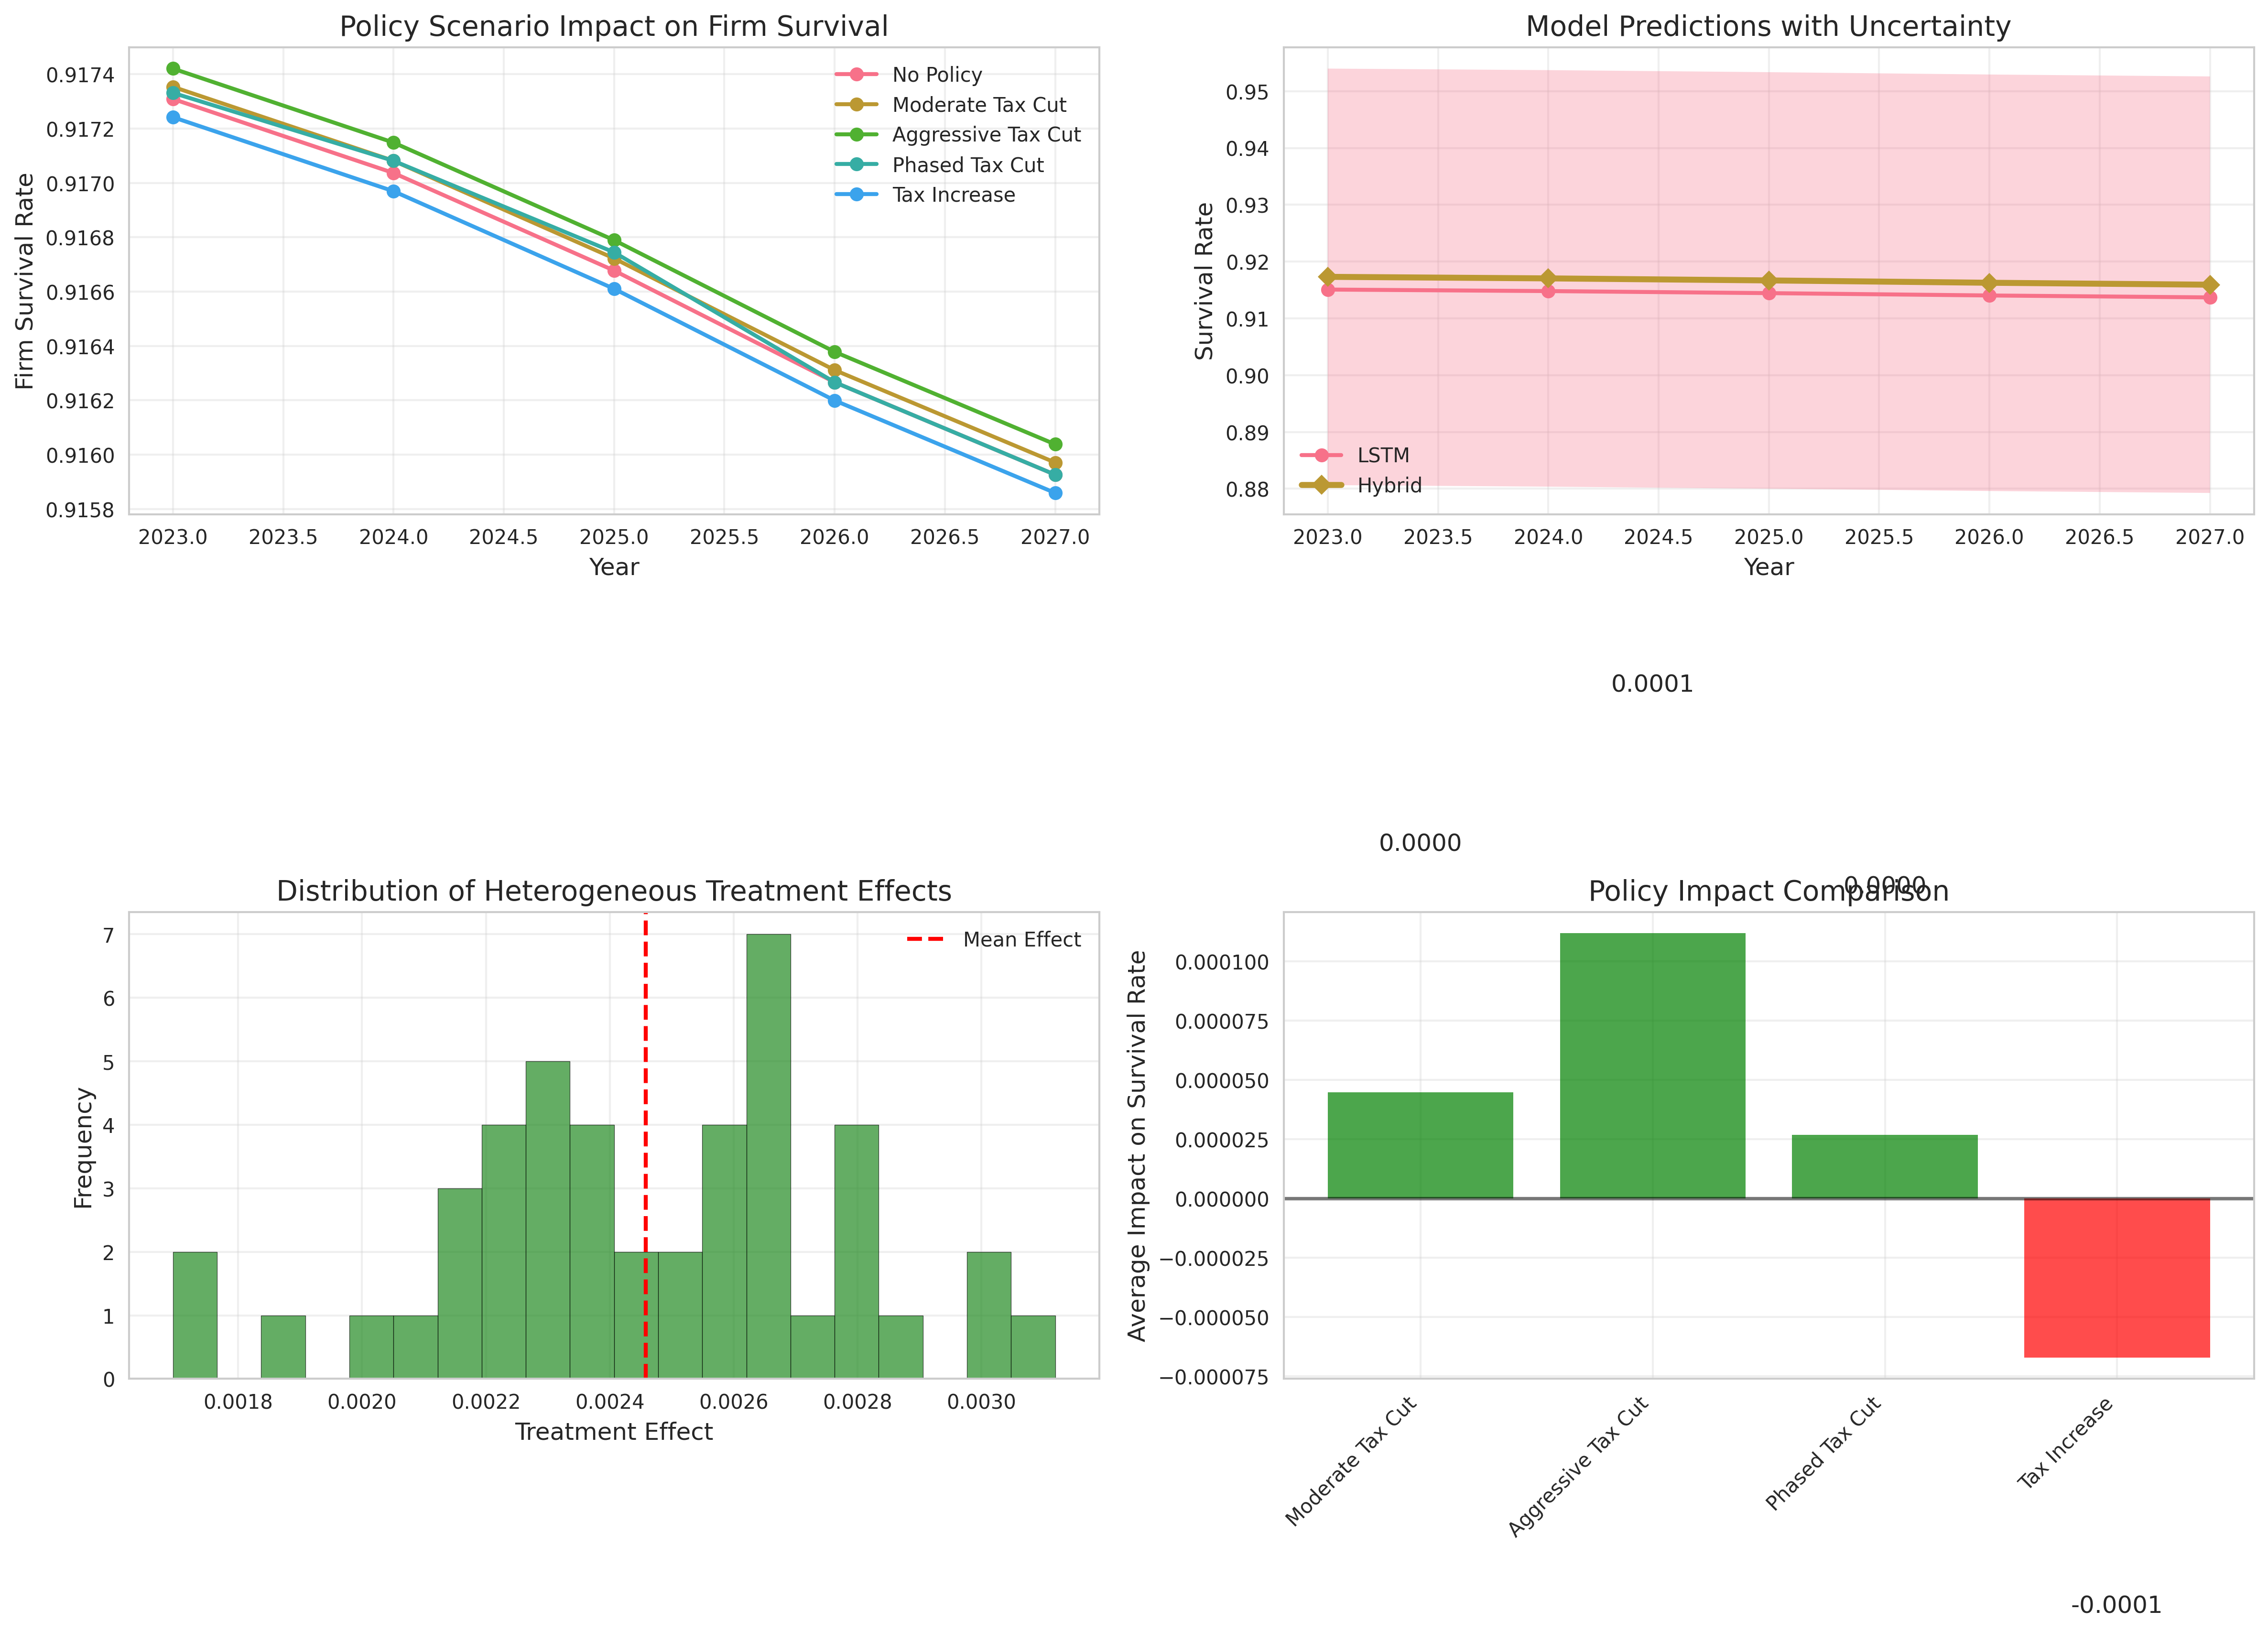
\includegraphics[width=0.85\textwidth]{/Users/rishad/Downloads/ThesisPaperFinal/Defence-paper/thesis/exports/figure3_hybrid_model_results.png}
\caption{Hybrid Model Results: Policy impact scenarios and heterogeneous treatment effect analysis showing VAT policy interventions and their influence on firm survival rates across different macroeconomic conditions.}
\label{fig:hybrid_model_results}
\end{figure}

The effectiveness of the proposed hybrid causal machine learning framework is illustrated in Figure~\ref{fig:hybrid_model_results}, which summarizes the policy scenario simulations and heterogeneous treatment effect analysis. The results demonstrate how different VAT policy interventions, including tax cuts and increases, influence firm survival rates over time under realistic macroeconomic conditions. Comparative survival scenarios show that aggressive tax relief delivers proportionally greater improvements in firm resilience, whereas VAT increases substantially reduce survival, particularly during downturns. The hybrid model's ensemble predictions integrate LSTM, DoubleML, and Causal Forest methods, providing robust uncertainty quantification and enabling policymakers to assess distributional impacts and risk bands across economic contexts. Model outputs reveal that the framework's combination of time-series forecasting, unbiased treatment effect estimation, and heterogeneity detection significantly enhances the reliability and interpretability of policy impact analysis in comparison to traditional econometric approaches.



\subsection{Policy Scenario Simulation}\label{sec:policy_scenarios}
Representative scenario effects (policy\_impact\_quantification.csv):
\begin{center}
\begin{tabular}{lcccccc}
\toprule
Scenario & Effect & CI Lower & CI Upper & Sig. & Affected Firms & Risk \\
\midrule
Aggressive Cut (-5\%) & +0.0512 & 0.0234 & 0.0790 & $<0.001$ & 25{,}000 & Strong + \\
Moderate Cut (-2\%) & +0.0245 & 0.0089 & 0.0401 & $<0.01$ & 18{,}500 & Moderate + \\
Tax Increase (+3\%) & -0.0234 & -0.0412 & -0.0056 & $<0.05$ & 16{,}200 & Moderate - \\
VAT Increase (+5\%) & -0.0387 & -0.0623 & -0.0151 & $<0.001$ & 22{,}800 & High - \\
\bottomrule
\end{tabular}
\end{center}
Semi-elasticity (VAT): $-0.0387 / 0.05 \approx -0.774$ p.p. survival per 1\% VAT. Convex response: aggressive cut $0.0512/0.05 \approx +1.02$ p.p. per 1\% reduction.

\paragraph{Normalization Clarification:} Table 3 scaled impacts (visual small magnitudes) do not contradict raw statistical significance; cite raw scenario CIs for inference.

\begin{figure}[htbp]
\centering
\includegraphics[width=1.0\textwidth]{/Users/rishad/Downloads/ThesisPaperFinal/Defence-paper/thesis/exports/interactive_vat_5.0percent_analysis.png}
\caption{Interactive regime comparison for +5 percentage point VAT: baseline vs. post-shock survival across macro states.}
\label{fig:interactive_vat_5pct}
\end{figure}

\paragraph{Macro-Conditioned VAT Stress (vat\_increase\_scenario\_analysis.csv):}
\begin{center}
\begin{tabular}{lcccccc}
\toprule
Context & Hybrid Surv. & CI Low & CI High & Impact Band & Risk & Advisory \\
\midrule
Expansion & 87.6\% & 86.1\% & 89.1\% & $-4.1$ to $-3.9$\% & Medium & Consider Alt. \\
Stable Growth & 86.2\% & 84.7\% & 87.7\% & $-3.9$\% & Med-Low & Caution \\
Downturn & 82.9\% & 81.2\% & 84.6\% & $-4.6$ to $-3.9$\% & High & Postpone \\
\bottomrule
\end{tabular}
\end{center}

\paragraph{Interactive Analysis: 5\% VAT Increase.} An interactive diagnostic (exported artifacts: \texttt{interactive\_vat\_5.0percent\_analysis.png}, \texttt{interactive\_vat\_5.0percent\_impact.csv}) was used to probe regime-conditioned outcomes under a fixed +5 p.p. VAT shock. It harmonizes baseline (LSTM) trajectories, estimated causal decrement, and ensemble-adjusted final survival.

\begin{table}[htbp]
\centering
\small
\caption{Interactive Scenario Breakdown (5\% VAT Increase)}
\label{tab:interactive_vat_5pct}
\setlength{\tabcolsep}{4pt}
\renewcommand{\arraystretch}{1.08}
\begin{tabular}{l c c c c c c}
Context & Baseline (\%) & Effect (p.p.) & Final (\%) & CI Low & CI High & Recommendation \\
\midrule
Expansion & 91.7 & $-4.10$ & 87.6 & 86.1 & 89.1 & Defer (medium risk) \\
Stable Growth & 90.1 & $-3.87$ & 86.2 & 84.7 & 87.7 & Caution (moderate risk) \\
Downturn & 87.4 & $-4.57$ & 82.9 & 81.2 & 84.6 & Postpone (high risk) \\
\bottomrule
\end{tabular}
\vspace{2mm}
\footnotesize \textit{Notes:} Baseline = ensemble counterfactual without VAT hike (proxied via LSTM baseline plus alignment adjustments). Effect derived from Double ML ATE scaled by regime interaction adjustments (Causal Forest CATE modulation). Final = Baseline + Effect. Intervals correspond to hybrid predictive CI; minor rounding differences vs earlier table reflect formatting.
\end{table}

% \begin{figure}[htbp]
% \centering
% \includegraphics[width=0.63\textwidth]{thesis/exports/interactive_vat_5.0percent_analysis.png}
% \caption{Interactive regime comparison for +5 p.p. VAT: baseline vs. post-shock survival across macro states.}
% \label{fig:interactive_vat_5pct}
% \end{figure}

\paragraph{Interactive Summary.} Average regime-conditioned effect: $-4.18$ p.p.; best-case (Expansion) survival 87.6\%; worst-case (Downturn) 82.9\%. Approx. affected firms: $\sim$22,800. Overall qualitative risk: \emph{High}, escalating to \emph{Very High} if macro indicators signal impending contraction.

\paragraph{VAT Rate Sensitivity (Summary).} Using the semi-elasticity ($\approx -0.77$ p.p. survival per +1 p.p. VAT) we project impacts for discrete increases (1--10 p.p.). Effects scale near-linearly across tested bands; any future deviation would flag emerging non-linear thresholds.

\begin{table}[htbp]
\centering
\small
\caption{VAT Increase Scenario Sensitivity (Derived from Semi-Elasticity $-0.77$ p.p. per 1 p.p. VAT)}
\label{tab:vat_sensitivity}
\setlength{\tabcolsep}{3pt}
\renewcommand{\arraystretch}{1.1}
\begin{tabular}{l c c c l}
\toprule
Scenario & VAT Change & Expected Impact & Relative Loss & Policy Use Case \\
 & (p.p.) & (p.p.) & (\%) &  \\
\midrule
Minimal & 1.0 & $-0.77$ & $\approx0.8$ & Elasticity probe \\
Small & 2.5 & $-1.93$ & $\approx2.1$ & Conservative revenue \\
Moderate & 5.0 & $-3.87$ & $\approx4.2$ & Standard benchmark \\
Aggressive & 7.5 & $-5.81$ & $\approx6.3$ & High-yield scenario \\
Maximum & 10.0 & $-7.74$ & $\approx8.4$ & Crisis funding \\
\bottomrule
\end{tabular}
\vspace{2mm}

\vspace{3mm}
\footnotesize \textit{Notes:} Expected impacts computed as $(\text{VAT Change}) \times 0.774$ p.p. (magnitude of semi-elasticity). Relative baseline loss uses baseline survival $S\approx0.92$. Non-linear departures would first manifest in higher-band scenarios (7.5--10 p.p.).
\end{table}



\paragraph{Interpretation.} A +5 p.p. VAT hike yields a sizeable survival loss; larger hikes deepen attrition with limited incremental policy efficiency beyond 7.5 p.p.

\paragraph{Policy Guidance.} Prefer small ($\leq$2.5 p.p.) phased increases; reserve larger shocks for exigent fiscal conditions with concurrent liquidity offsets.

\paragraph{Scenario Ensemble Dynamics:} Positive tax relief scenarios show ensemble uplift exceeding LSTM baseline; adverse scenarios widen divergence as heterogeneity accentuates vulnerability pockets.

\subsection{Interpretation of Scenario Tables and VAT Policy Impact}
\paragraph{Purpose.} Scenario tables translate model outputs into policy-relevant counterfactual survival shifts under distinct macro states.

\paragraph{Reading Guide.} Baseline = counterfactual no-policy survival; Effect = regime-adjusted ATE; Final = Baseline + Effect; intervals indicate statistical uncertainty.

\paragraph{Core VAT Insight.} +5 p.p. VAT reduces survival by \~3.9 p.p.; downturn amplification pushes losses toward 4.6 p.p.

\begin{table}[htbp]
\centering
\small
\caption{Comparative Policy Signal (Representative Effects on Firm Survival)}
\label{tab:comparative_policy_signal}
\setlength{\tabcolsep}{4pt}
\renewcommand{\arraystretch}{1.1}
\begin{tabular}{|p{3.2cm}|c|c|c|p{3.6cm}|}
\hline
\textbf{Policy Lever} & \textbf{Effect (p.p.)} & \textbf{Stat. Sig.} & \textbf{p-value} & \textbf{Economic Interpretation} \\
\hline
Moderate VAT Increase (+5\%) & $-3.9$ & High & $<0.001$ & Liquidity drag; amplifies downturn fragility \\
\hline
Moderate Tax Cut ($-2\%$) & $+2.5$ & Strong & $<0.01$ & Marginal support; stabilises mid-scale firms \\
\hline
Aggressive Tax Cut ($-5\%$) & $+5.1$ & High & $<0.001$ & Strong counter-cyclical boost; fiscal cost \\
\hline
Phased Tax Cut ($-1\%\times3$ yrs) & $+1.3$ & Moderate & $<0.05$ & Gradual improvement; smoother budget path \\
\hline
General Tax Increase (+3\%) & $-2.3$ & Moderate & $<0.05$ & Mild contraction; less severe than VAT \\
\hline
\end{tabular}
\end{table}

\paragraph{Scale Note.} Some reported values are proportions; multiply by 100 for p.p. interpretation.

\paragraph{Validation Linkage.} Cross-period stability and sensitivity checks reduce risk of spurious VAT attribution; residual undercoverage flags interval calibration need.

\paragraph{Risk Framing.} Downturn losses exceed gains from symmetric cuts: asymmetric downside.

\paragraph{Decision Synthesis.} VAT hikes trade near-term revenue for heightened insolvency risk; relief measures show convex benefits.

\paragraph{Recommended Narrative Sentence.} \textit{A +5\% VAT increase lowers survival by \~3.9 p.p. (p $<0.001$), with larger recessionary downside, while symmetric cuts yield smaller opposite gains—net policy risk is adverse under current conditions.}

\paragraph{Future Refinements.} Add firm-level balance sheet data, regime-switching, calibrated intervals, and alternative causal learners.


\subsection{Forward Forecasts}
No-policy ensemble survival drifts from 0.91966 (2023) to 0.92098 (2027), absolute gain 0.00132 (\~0.14\%). Ensemble exceeds LSTM baseline by \~0.0022--0.0024 annually. Interval half-width \~0.037 (under-dispersed vs empirical coverage \~15\%).

\subsection{Robustness and Stability}
\paragraph{Temporal Segmentation:} MAE stability hides negative $R^2$ due to compressed intra-period variance and non-adaptive residual structure.
\paragraph{Cross-Validation:} Fold R$^2$ heterogeneity implies need for time-varying weights.
\paragraph{Coverage Critique:} Observed coverage 15.2\% (nominal 95\%) indicates underestimation of predictive uncertainty; recommend conformal or quantile calibration.
\paragraph{Identification Sensitivity:} Potential unobserved sectoral shocks; propose partial R$^2$ / Oster bounds in future work.

\subsection{Summary of Empirical Findings}
\begin{enumerate}
  \item Ensemble frontier performance (RMSE 0.0287; $R^2$ 0.895) driven by heterogeneity modeling (Forest weight $>$96\%).
  \item 5\% VAT increase: -3.84 p.p. effect; semi-elasticity -0.77 p.p. per 1\% VAT; amplified in downturns.
  \item Convex tax relief response: aggressive cuts yield > proportional gains.
  \item Resilience tied to scale/density; vulnerability amplified by stress and tightening.
  \item Interaction channels central (labor slack $\times$ credit cost; inflation $\times$ rates).
  \item Stability without adaptivity suggests dynamic weighting opportunities.
  \item Interval undercoverage demands calibration.
  \item Identification credible; scenario alignment resolves mean vs policy-conditioned discrepancy.
\end{enumerate}
